
\section*{Pruebas de Laboratorio Alta Tensión}

Para probar el funcionamiento de un transformador, es necesario someterlo a un par de pruebas, las cuales son la Prueba de Corto Circuito y la Prueba de Circuito Abierto. Con base en estas dos pruebas podemos ver la relación de tensión entre ambos bobinados, las corrientes que manejan estos y su potencia.

\subsection*{Prueba de Corto Circuito}

Para esta prueba, se cortocircuita uno de los lados del transformador. Se calcula qué corriente pasa por este cortocircuito y qué tensión es la aplicada en el lado primario. Al escoger una potencia de 50 W y tener el lado secundario con una tensión de 50 V, se aplica una corriente por el cortocircuito de 1 A. Por la fórmula (sabiendo que la potencia reactiva de la rama de magnetización es muy ínfima):
\begin{figure}[ht!]
    \centering
    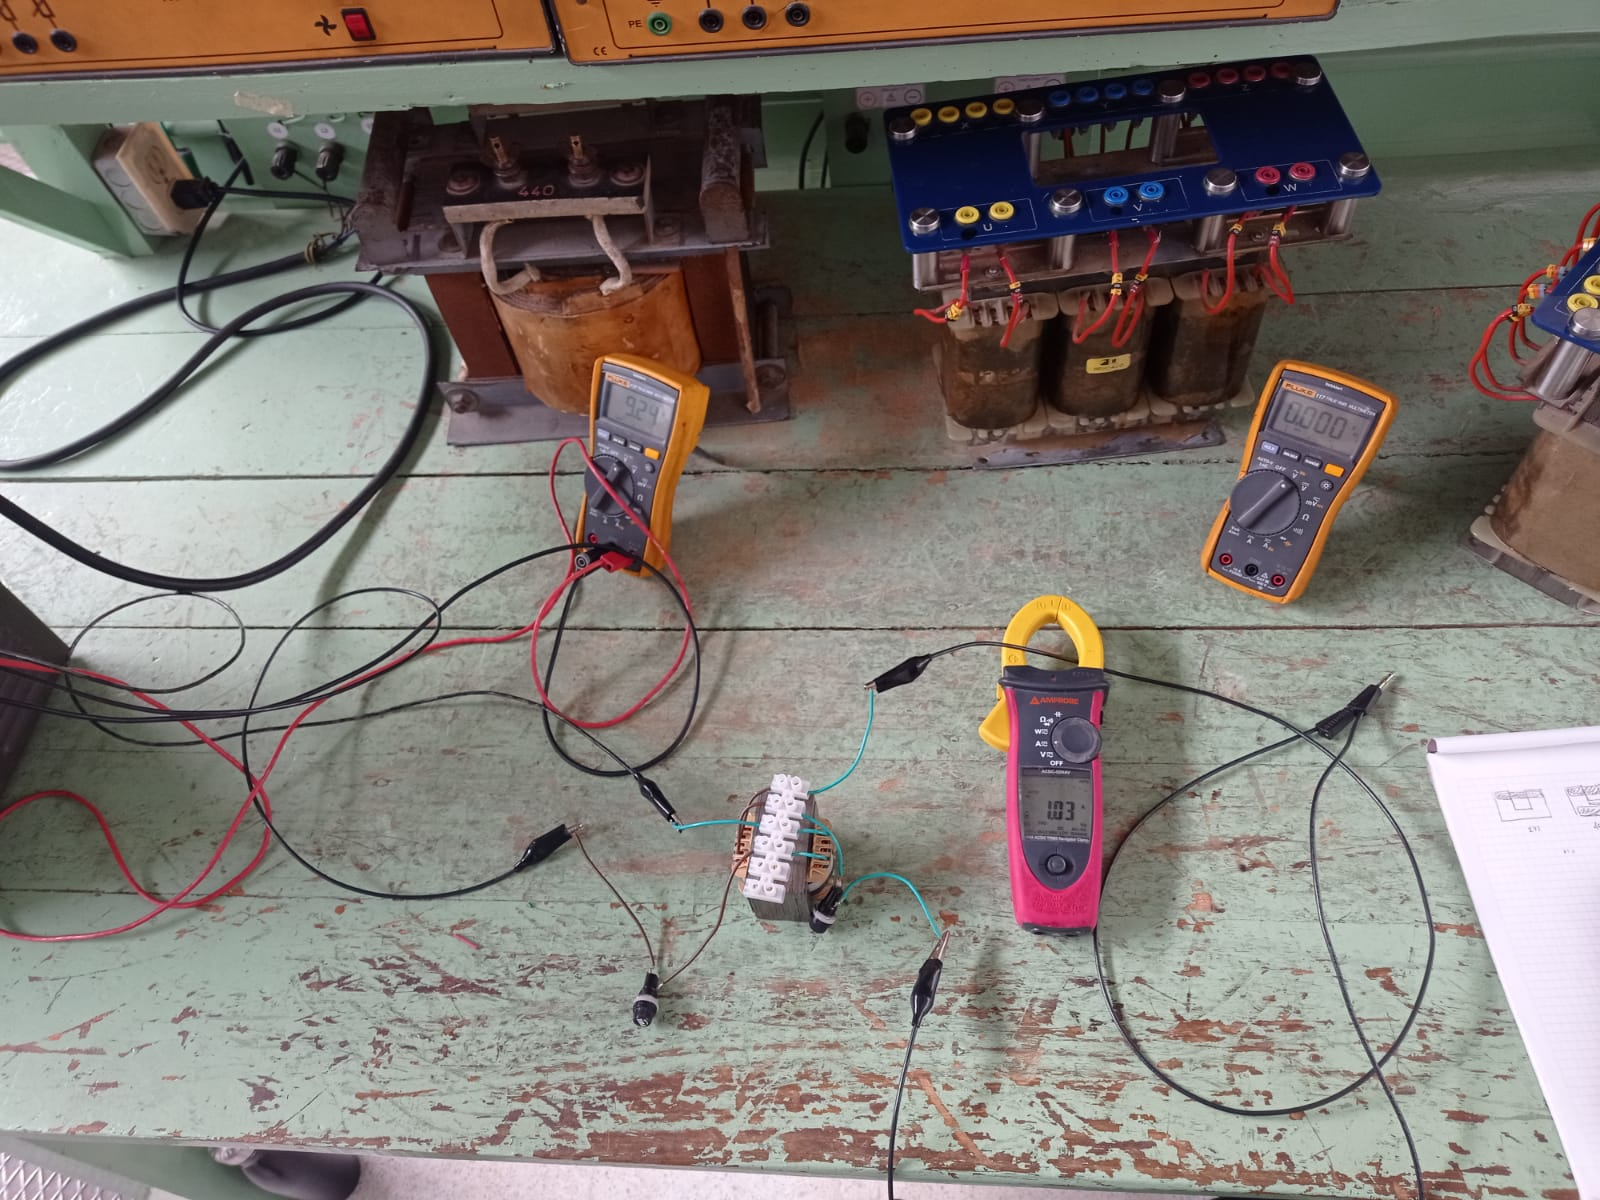
\includegraphics[width=0.48\textwidth]{fot/TP1.jpeg}
    \caption{Prueba en el laboratorio de alta tensión.}
    \label{fig:TP1}
\end{figure}

\begin{center}
    $S = V \cdot I = 50\ [VA]$
\end{center}
Tensión del lado primario:
\begin{center}
    $9.24 [V]$
\end{center}

\begin{center}
    $Corriente \ que \ recorre \ el \ cortocircuito: \ 1.03\ [A]$
\end{center}

\subsection*{Prueba de Circuito Abierto}

En esta prueba, se deja el lado secundario abierto. Se calcula la tensión en este lado y se toman la corriente y la tensión que aplicamos en el lado primario del transformador. Para esta parte del laboratorio se comprueba la relación de transformación, teniendo en cuenta los criterios que escogimos para nuestro transformador, el cual es: tensión del lado primario 120 V y lado secundario 50 V. Aplicamos la fórmula:

Relación de transformación:
\begin{center}
    $\frac{V_p}{V_s} = \frac{120\ [V]}{50\ [V]} = 2.4$
\end{center}


\begin{figure}[ht!]
    \centering
    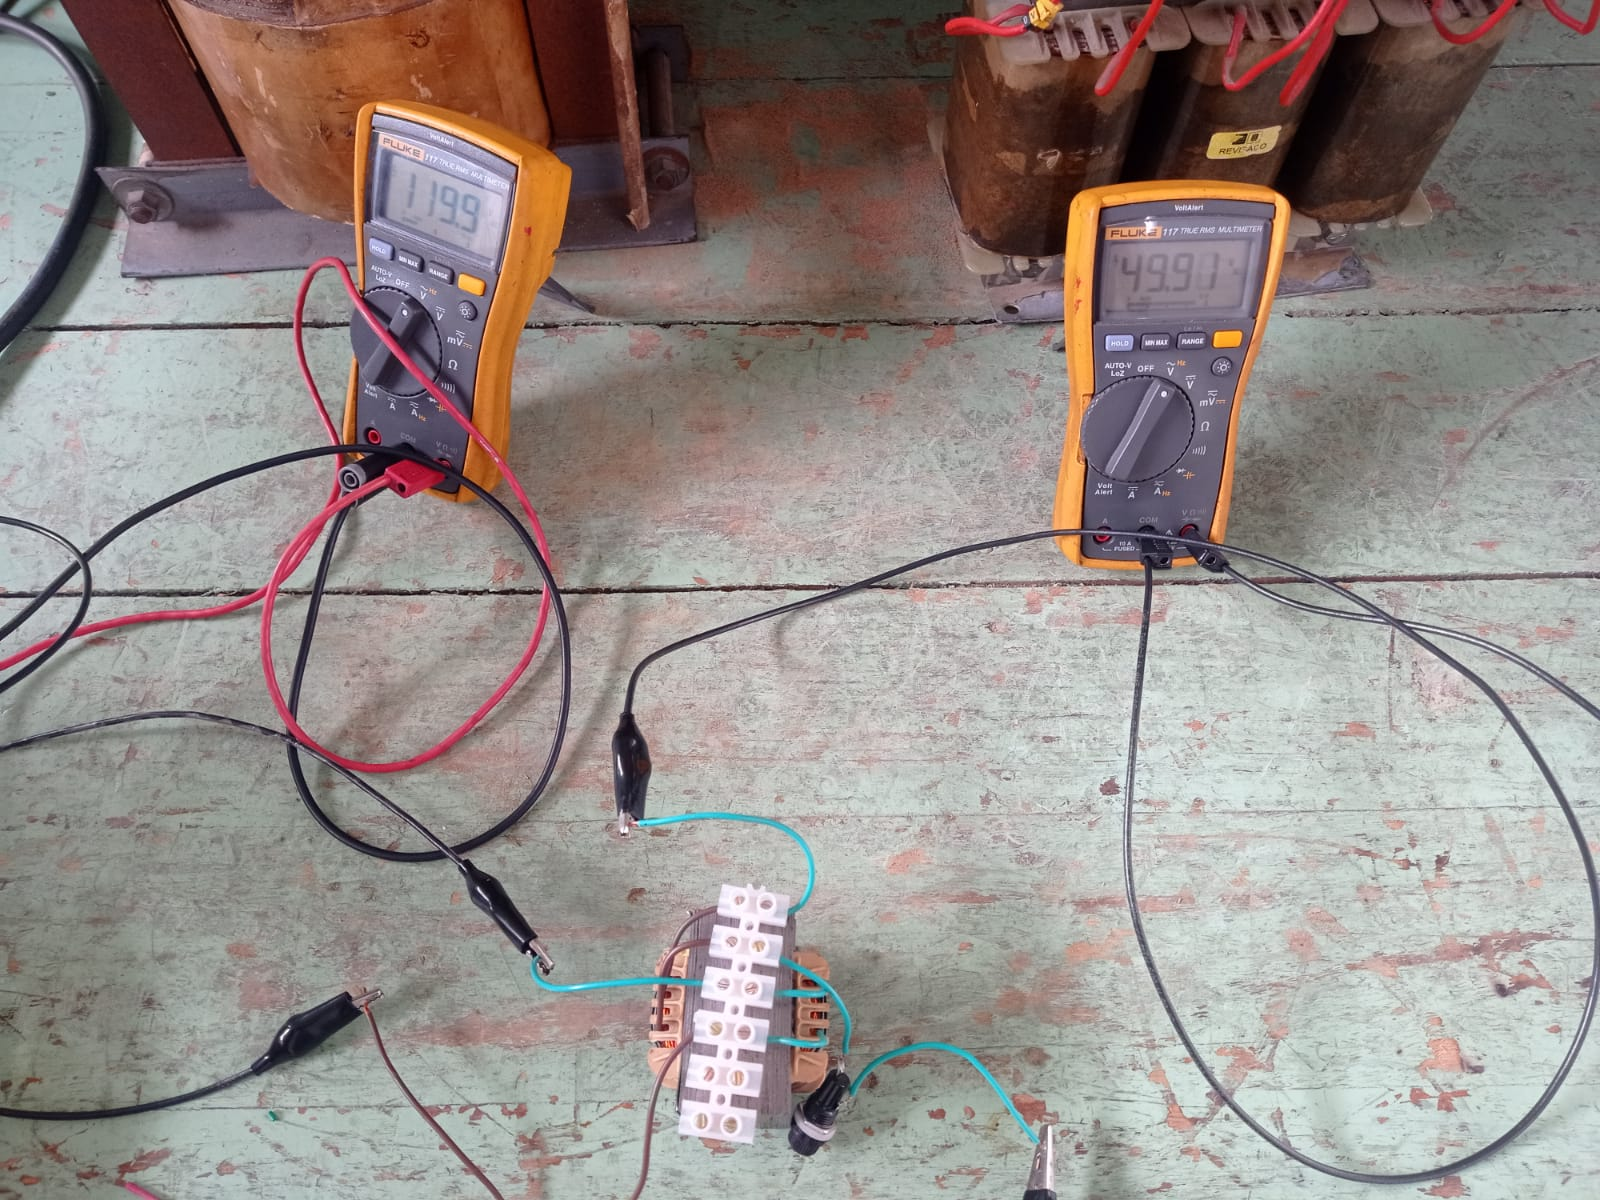
\includegraphics[width=0.48\textwidth]{fot/TP3.jpeg}
    \caption{Prueba en el laboratorio de alta tensión.}
    \label{fig:TP3}
\end{figure}
 
Tensión en el lado primario del transformador:
\begin{center}
    $119.9\ [V]$
\end{center}
Tensión en el lado secundario del transformador: 
\begin{center}
    $49.91\ [V]$
\end{center}
Relación de transformación: 
\begin{center}
    $ \frac{119.9\ [V]}{49.91\ [V]} = 2.402$
\end{center}
Corriente por el lado primario del transformador: 
\begin{center}
    $0.22\ [A]$
\end{center}
\begin{figure}[ht!]
    \centering
    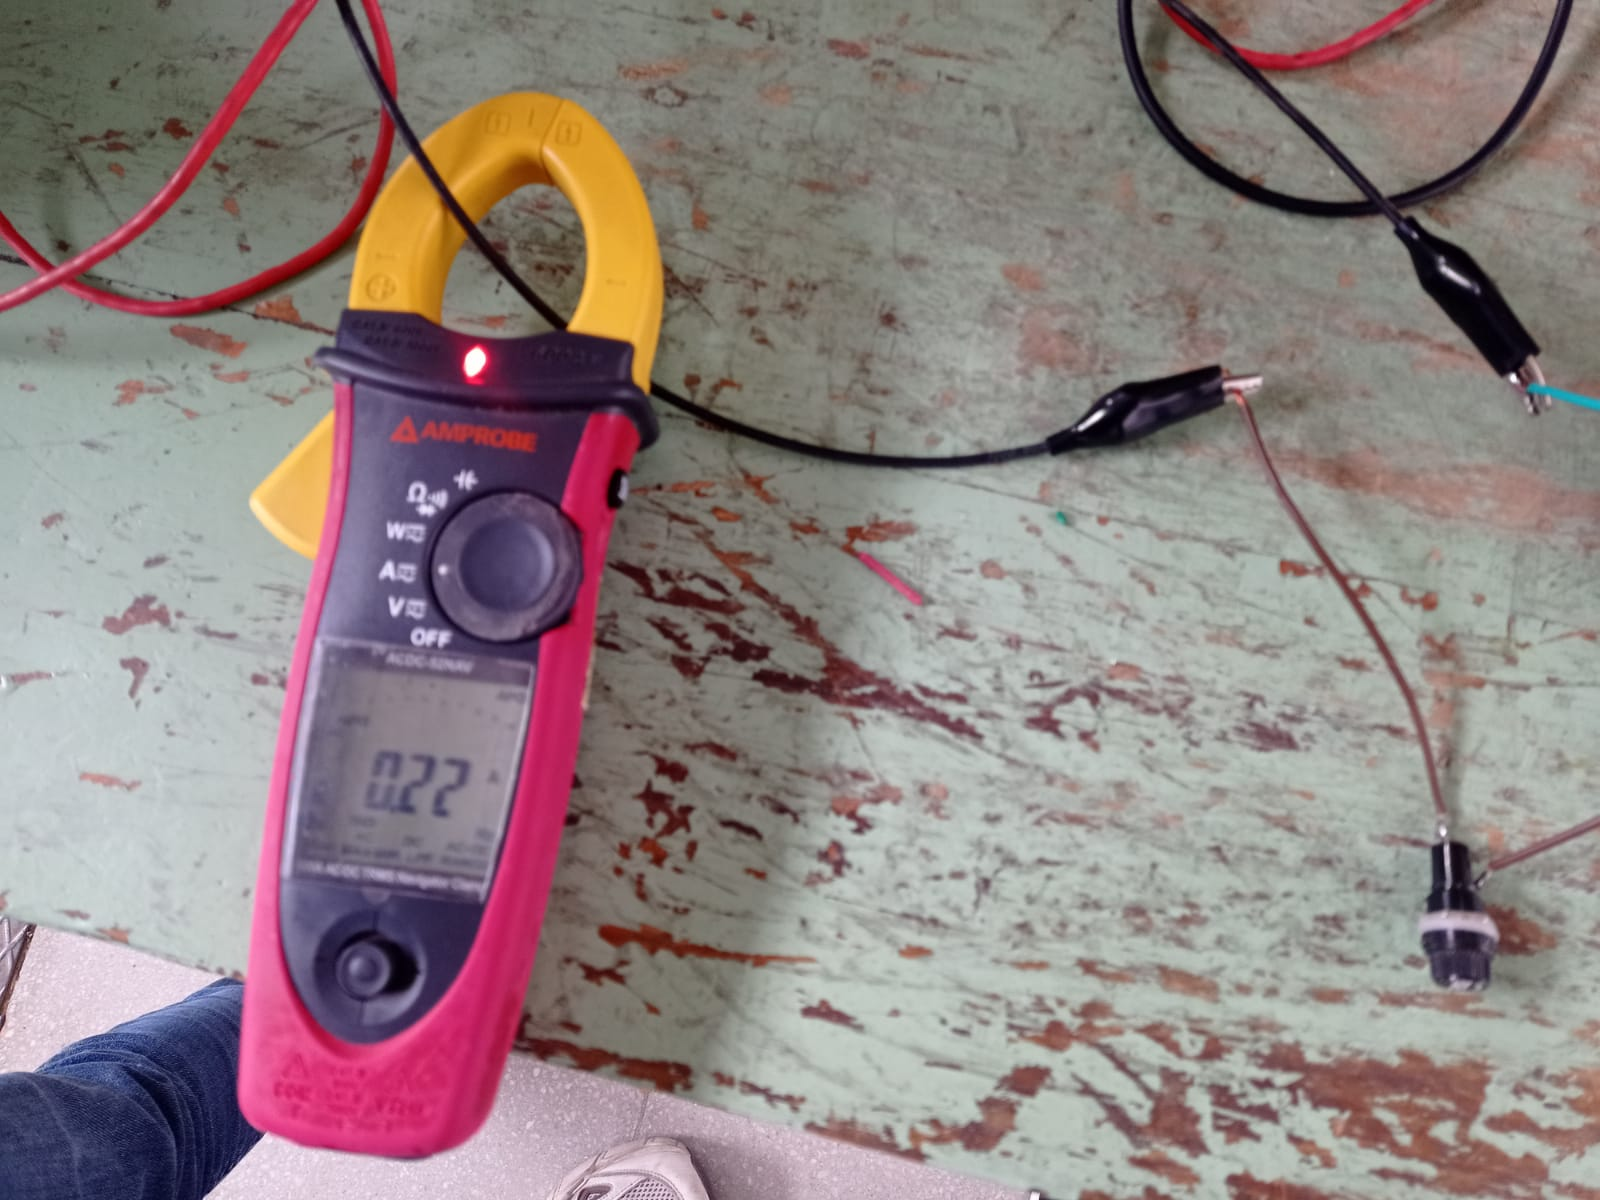
\includegraphics[width=0.48\textwidth]{fot/TP2.jpeg}
    \caption{Prueba en el laboratorio de alta tensión.}
    \label{fig:TP2}
\end{figure}


\section{analisis de resultados}
\subsection{Resultados de la prueba de circuito abierto}
Al realizar la prueba de circuito abierto, se observa que la tensión en el lado primario es de 119.9 V y la tensión en el lado secundario es de 49.91 V, lo que indica que la relación de transformación es de 2.402. Esto significa que el transformador está funcionando correctamente y que la relación de transformación es la esperada.
Con relación a la corriente de excitación en el lado primario es de 0.22 A, de la cual para valores nominales se esperaba que fuera de 0,4166 A. para lo cual se tiene que la corriente de excitación es 52.8\% lo quiere decir que la rama de magnetización tiene un valor por encima del esperado que es del 10\% respecto a la nominal%.

\subsection{Resultados de la prueba de corto circuito}
Al realizar la prueba de corto circuito, se observa que la tensión en el lado primario es de 9.24 V y la corriente en el lado del cortocircuito es de 1.03 A. Esto indica que el transformador está funcionando correctamente. Para la corriente de carga para valores nominales se tendria ques deberia ser de 1[A] por lo cual respecto a esta se tiene que la corriente de carga es del 103\% respecto a la nominal. Esto indica que el transformador está funcionando correctamente en los valores esperados.


\section{Conclusiones}
\begin{itemize}
    
    \item En cuanto a la relación de transformación, el transformador presenta valores esperados, lo que indica que el transformador está funcionando correctamente.
    \item La potencia nominal del transformador es de 50 VA, lo que indica que el transformador está diseñado para manejar esta potencia sin problemas y que no se espera que se produzcan sobrecalentamientos o fallas en el transformador si se dimensiona un uso para estos valores.
    \item El transformador presenta valores por encima de lo esperado para la corriente de la rama de magnetización esto podría deberse a los ciclos de histéresis y corrientes parásitas principalmente el primer caso, lo que provoca que la corriente de excitación sea mayor a la esperada. 
    \item La corriente de carga es del 103\% respecto a la nominal, lo que indica que el transformador está funcionando correctamente en los valores esperados.
    \item S\item En cuanto a la relación de transformación, el transformador presenta valores esperados, lo que indica que el transformador está funcionando correctamente.e logro comprender satisfactoriamente el funcionamiento del transformador, así como su diseño y construcción. lo que a futuro nos permitiria reallizar uno en funcion de las necesidades de un circuito en particular.
\end{itemize}






\section{Anexos}
\subsection{Imágenes de la construcción del transformador}
Las imagenes de la construcción del transformador son las figuras \ref{fig:TA1} a \ref{fig:TA6}.
\begin{figure}[ht!]
    \centering
    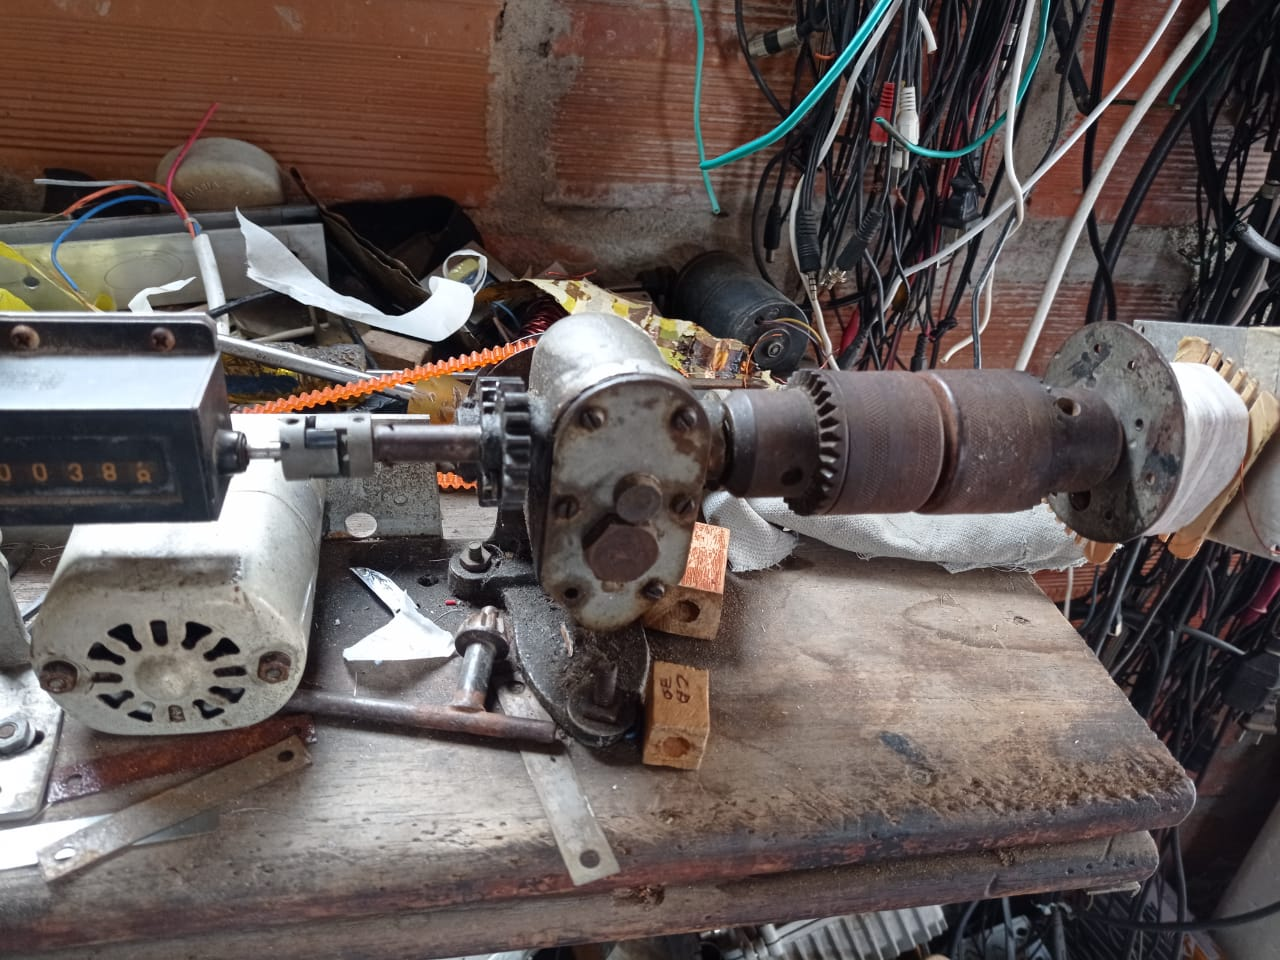
\includegraphics[width=0.48\textwidth]{fot/TA1.jpg}
    \caption{Construcción del transformador con el numero de vueltas del devanado primario mas cinta de enmascarar.}
    \label{fig:TA1}
\end{figure}

\begin{figure}[ht!]
    \centering
    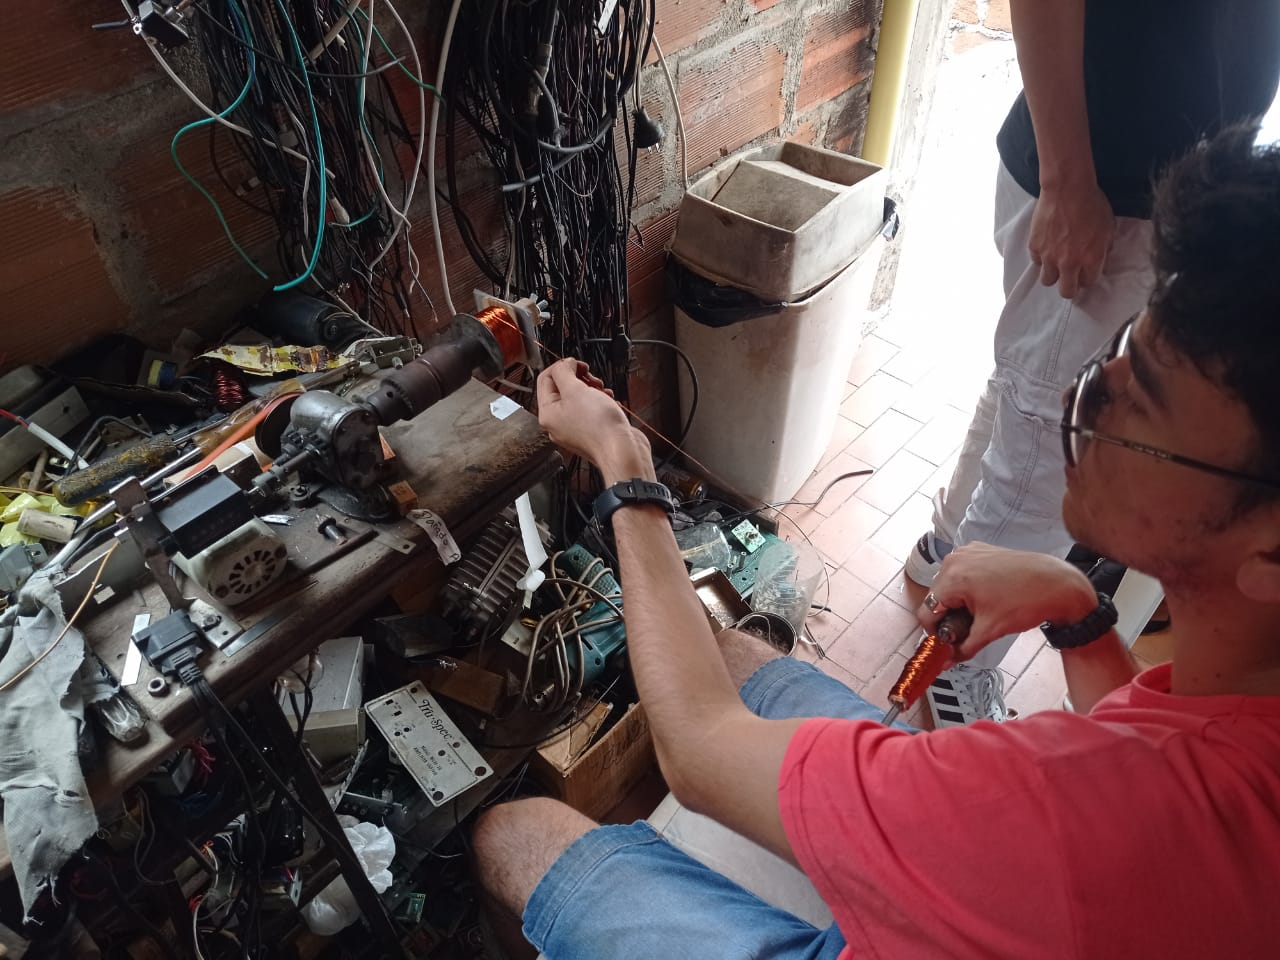
\includegraphics[width=0.48\textwidth]{fot/TA2.jpeg}
    \caption{Construcción del transformador.}
    \label{fig:TA2}
\end{figure}

\begin{figure}[ht!]
    \centering
    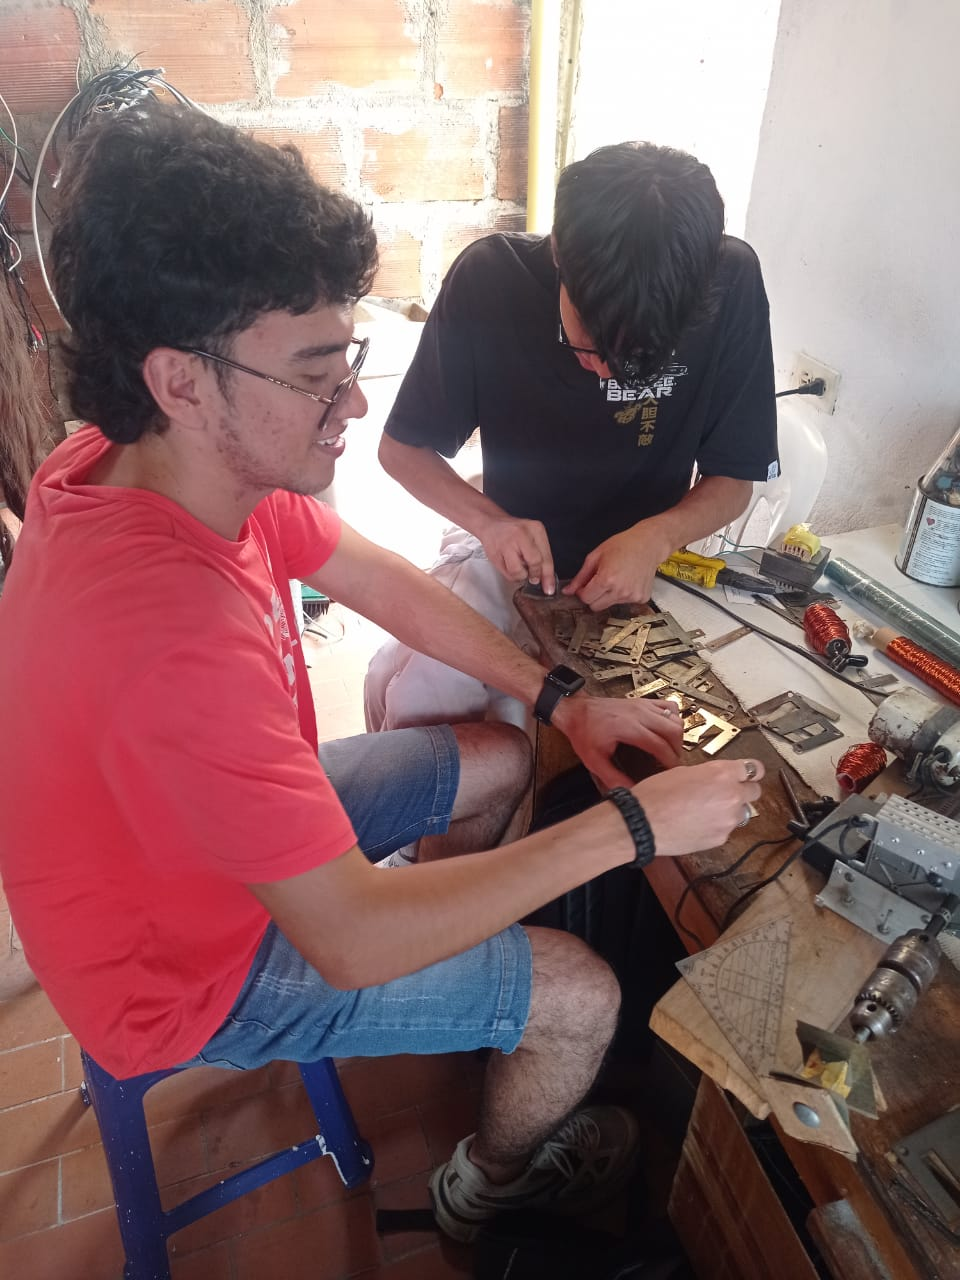
\includegraphics[width=0.48\textwidth]{fot/TA3.jpeg}
    \caption{Construcción del transformador .}
    \label{fig:TA3}
\end{figure}

\begin{figure}[ht!]
    \centering
    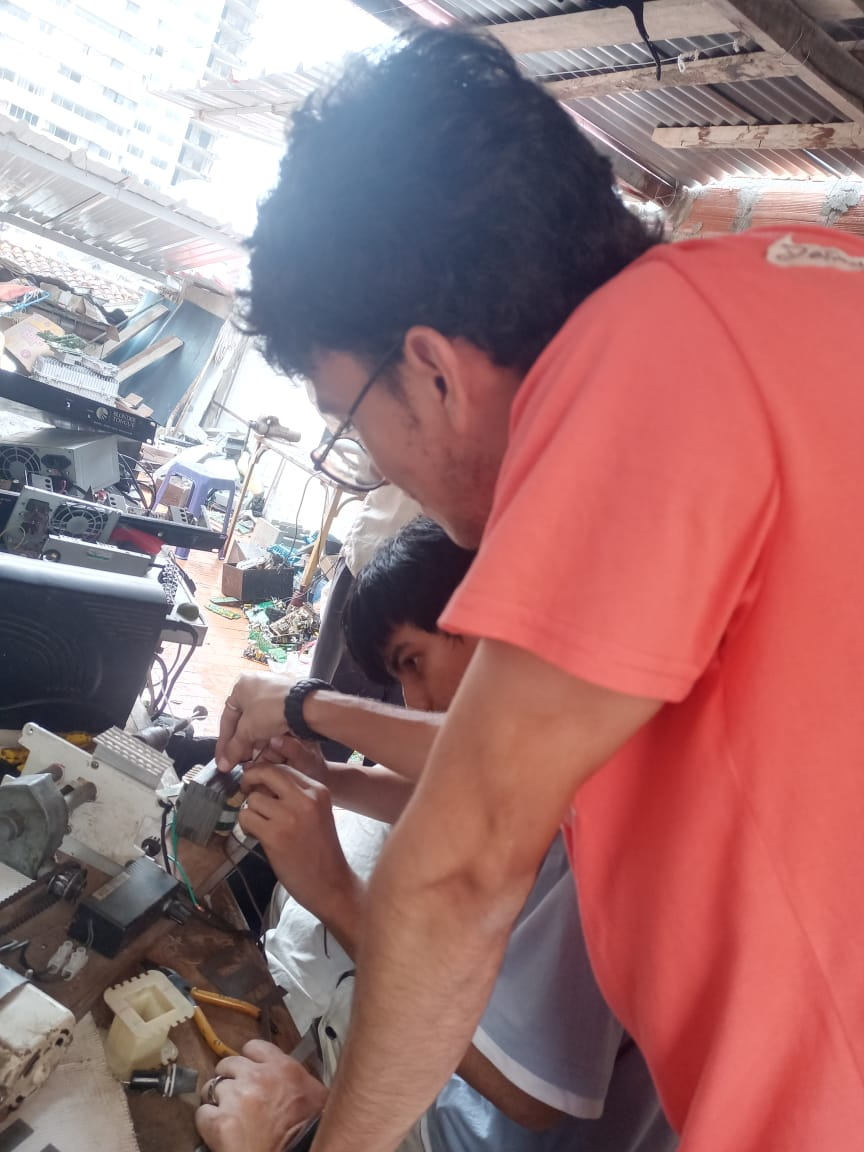
\includegraphics[width=0.48\textwidth]{fot/TA4.jpeg}
    \caption{Construcción del transformador.}
    \label{fig:TA4}
\end{figure}

\begin{figure}[ht!]
    \centering
    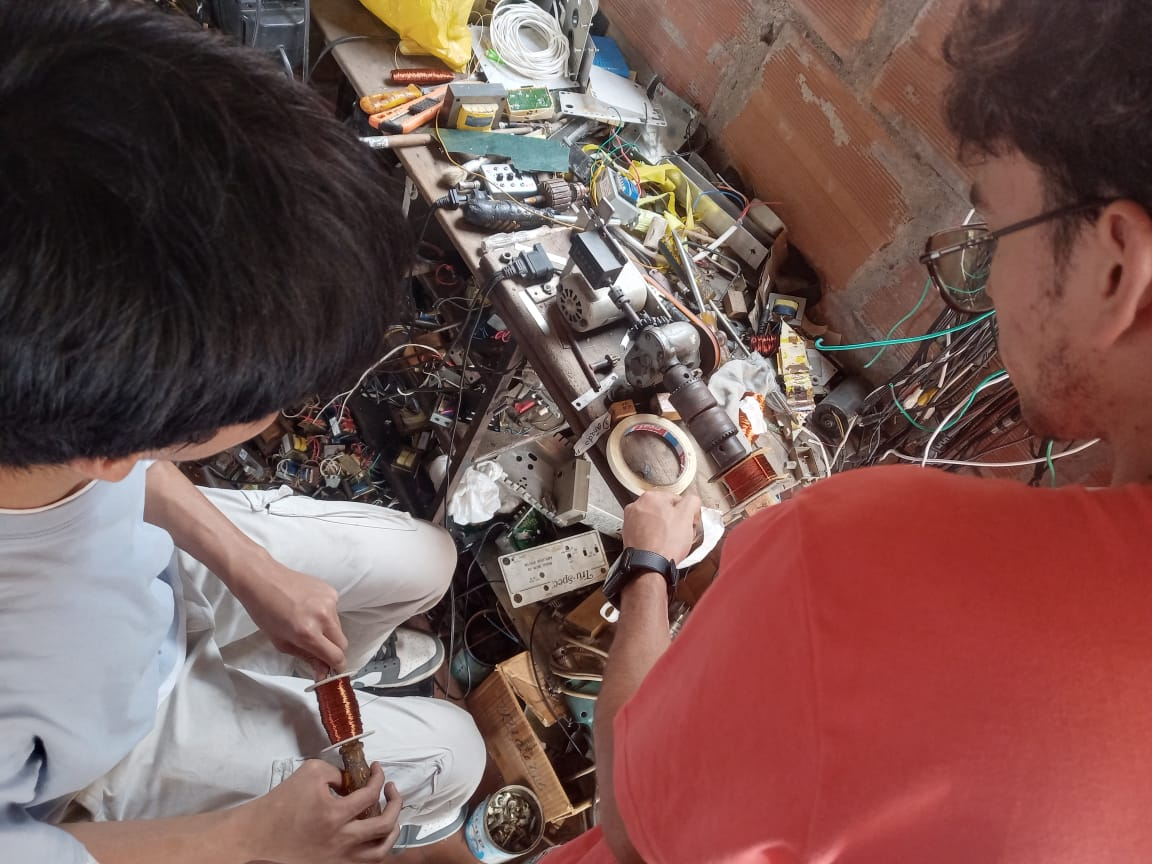
\includegraphics[width=0.48\textwidth]{fot/TA5.jpeg}
    \caption{Construcción del transformador.}
    \label{fig:TA5}
\end{figure}

\begin{figure}[ht!]
    \centering
    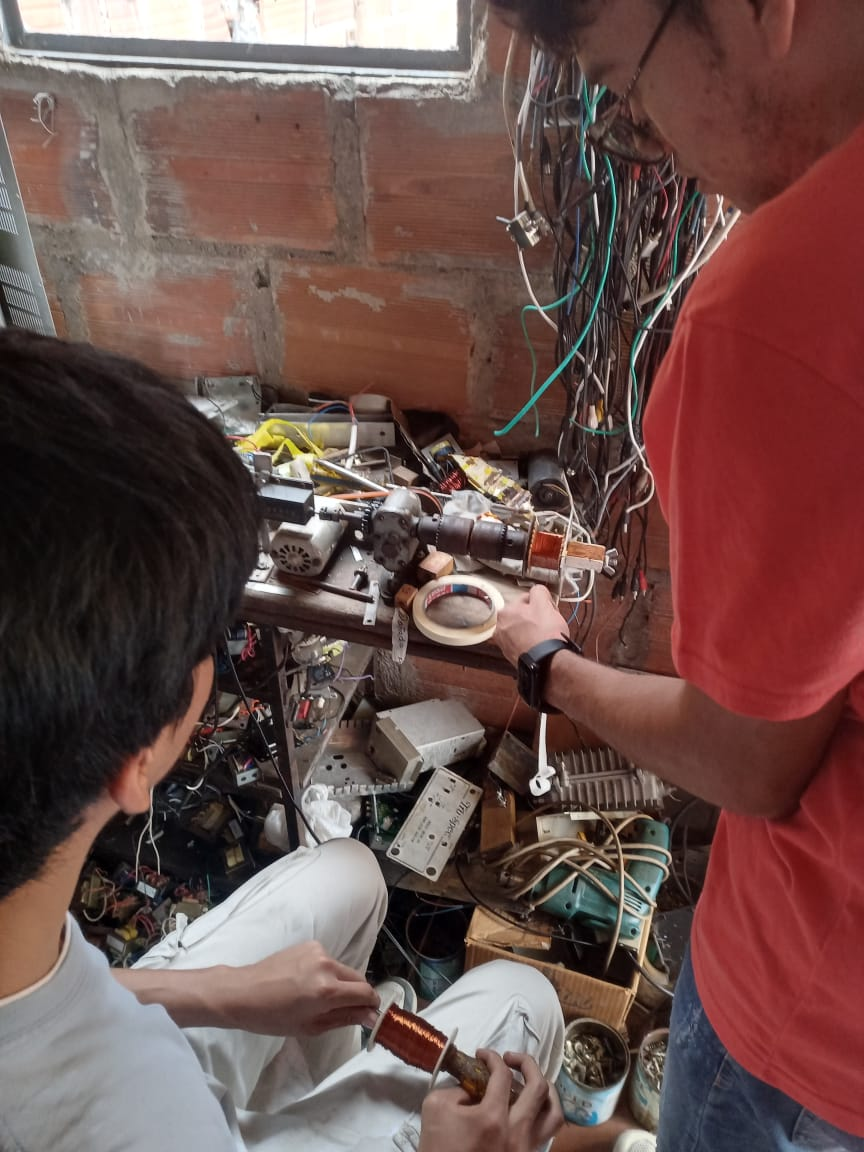
\includegraphics[width=0.48\textwidth]{fot/TA6.jpeg}
    \caption{Construcción del transformador.}
    \label{fig:TA6}
\end{figure}
